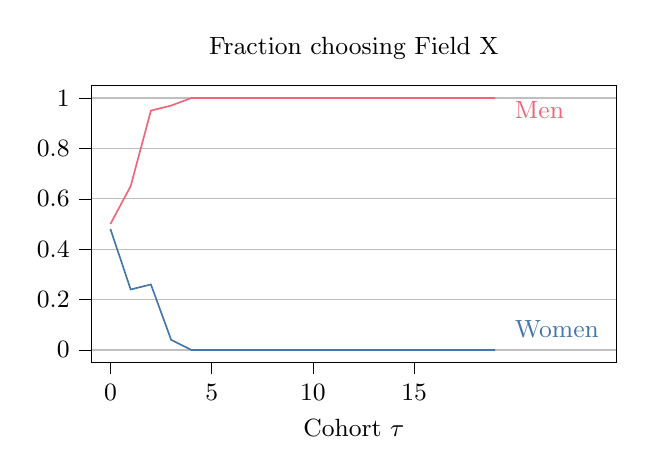
\begin{tikzpicture}[every node/.style={font=\small}]
% This file was created with tikzplotlib v0.9.17.
\definecolor{color0}{rgb}{0.266666666666667,0.466666666666667,0.666666666666667}
\definecolor{color1}{rgb}{0.933333333333333,0.4,0.466666666666667}

\begin{axis}[
height=5.101085673964669cm,
tick align=outside,
tick pos=left,
title={Fraction choosing Field X},
width=8.25373cm,
x grid style={white!69.0196078431373!black},
xlabel={Cohort \(\displaystyle \tau\)},
xmin=-0.95, xmax=25,
xtick style={color=black},
xtick={0,5,10,15},
xticklabels={
  \(\displaystyle 0\),
  \(\displaystyle 5\),
  \(\displaystyle 10\),
  \(\displaystyle 15\)
},
ymajorgrids,
ymin=-0.05, ymax=1.05,
ytick style={color=black},
ytick={-0.2,0,0.2,0.4,0.6,0.8,1,1.2},
yticklabels={
  \(\displaystyle -0.2\),
  \(\displaystyle 0\),
  \(\displaystyle 0.2\),
  \(\displaystyle 0.4\),
  \(\displaystyle 0.6\),
  \(\displaystyle 0.8\),
  \(\displaystyle 1\),
  \(\displaystyle 1.2\)
}
]
\addplot [semithick, color0]
table {%
0 0.480000019073486
1 0.240000009536743
2 0.259999990463257
3 0.0399999618530273
4 0
19 0
};
\addplot [semithick, color1]
table {%
0 0.5
1 0.649999976158142
2 0.950000047683716
3 0.970000028610229
4 1
19 1
};
\draw (axis cs:19.5,0.05) node[
  anchor=base west,
  text=color0,
  rotate=0.0
]{Women};
\draw (axis cs:19.5,0.92) node[
  anchor=base west,
  text=color1,
  rotate=0.0
]{Men};
\end{axis}



\end{tikzpicture}